\section{Stereo Matching - needs work done}

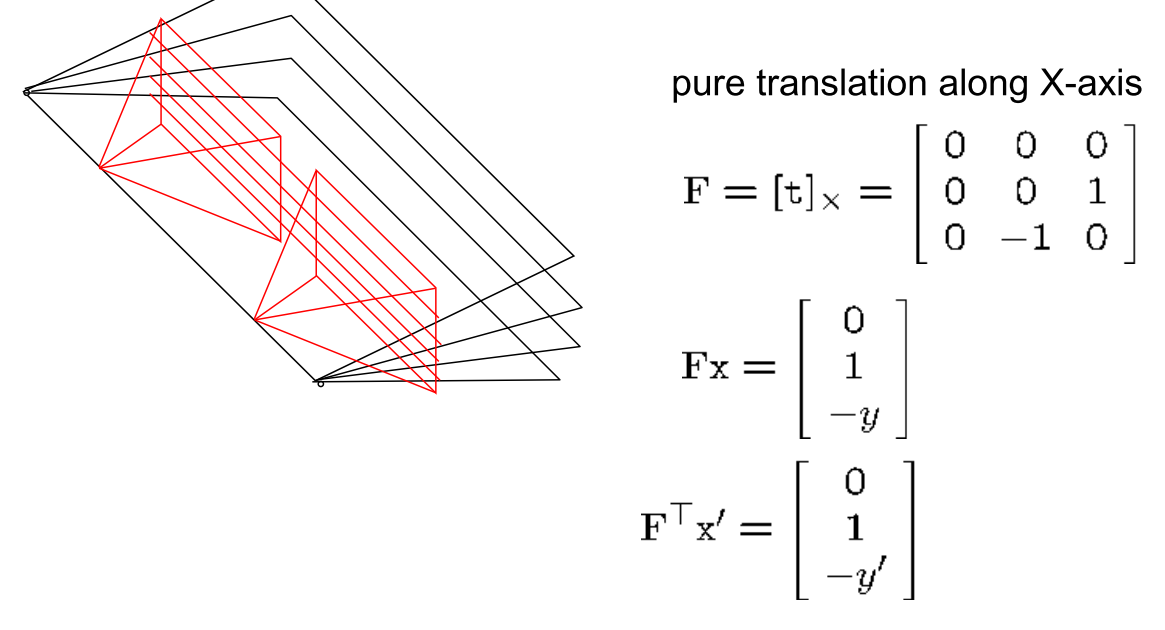
\includegraphics[width=\columnwidth]{pictures/standardstereo}


\subsection{Occlusion}
In an image pair each pixel has at most one corresponding pixel – In general one corresponding pixel – In case of occlusion there is none

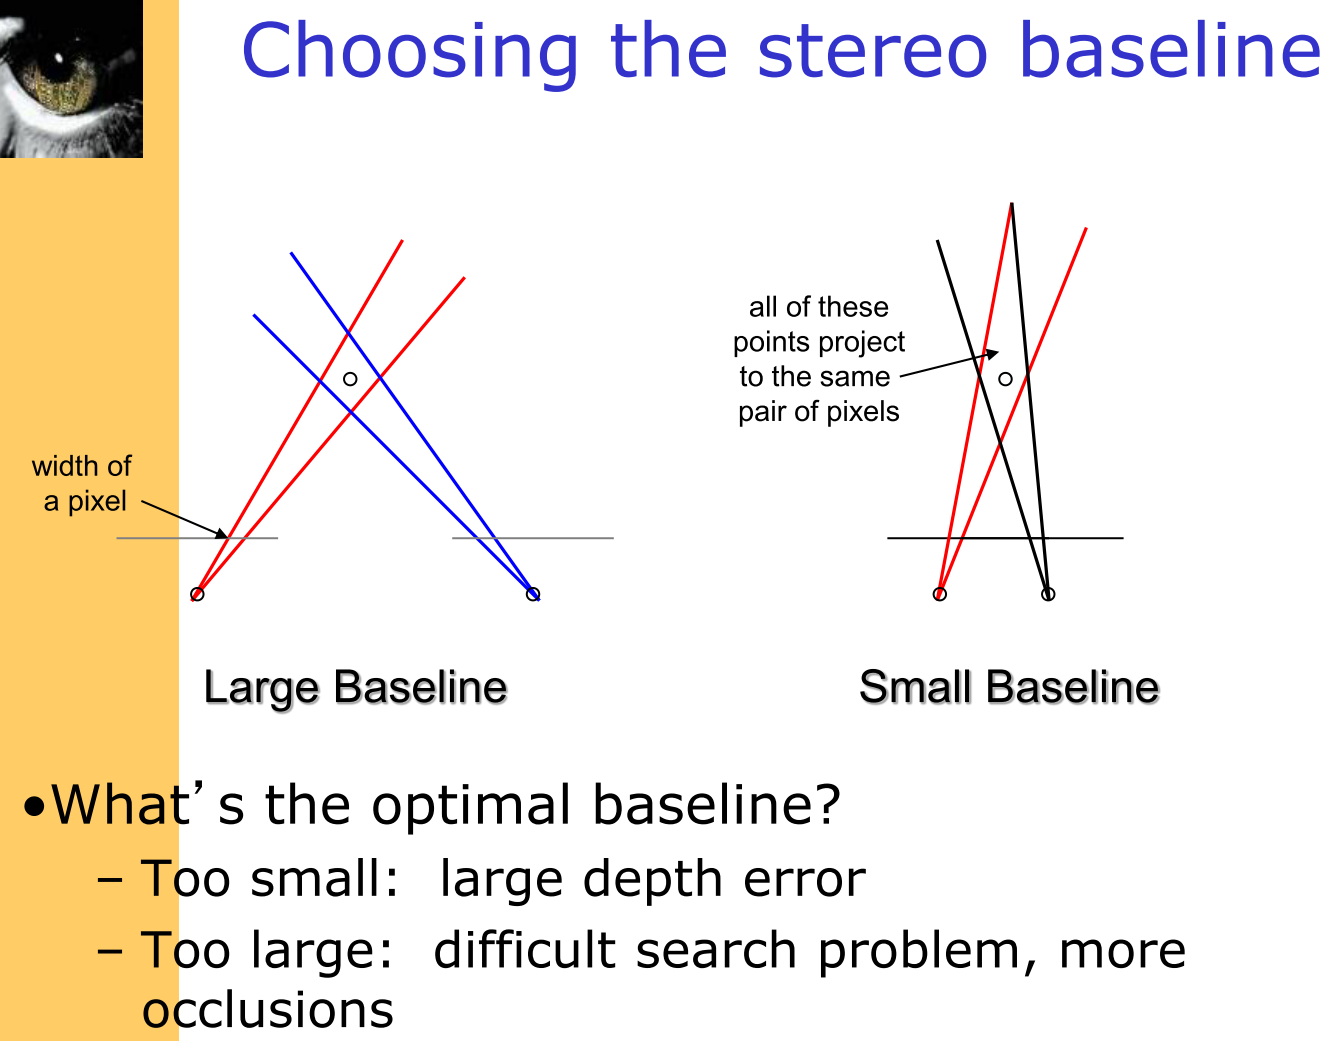
\includegraphics[width=\columnwidth]{pictures/stereobaseline}

\subsection{Deep Stereo Matching}


\subsection{3D convex hull}
The 3D convex hull of a set of 3D points is the smallest convex set which contains all 3D points.

\subsection{Visual hull}
The visual hull is the smallest volume which can be obtained by intersecting the generalized cones generated by all possible 2D shape projections ofa 3D object.\\
\\
In 3D, the visual hull is a subset ofthe convex hull. 

\subsubsection{voxel-base, marching intersections, exact polyhedral}

\subsection{Photo hull}
The photo hull is the union ofall photo-consistent volumes and the tightest possible bound on the true scene.\\
\\
It is a subset of the visual hull and - in contrast to the 3D convex hull and the visual hull depends on the texture of the 3D object.
\subsubsection{Voxel coloring}

\subsubsection{Space Carving}

Step 1: Initialize V to volume containing true scene\\
Step 2: For every voxel on surface of V test photo-consistency of voxel if voxel is inconsistent, carve it\\
Step 3: Repeat Step 2 until all voxels consistent\\
\\

Convergence: Always converges to a photo-consistent model (when all assumptions are met)
Good results on difficult real-world scenes\\
\\
Properties of Volume Intersection\\
Pros – Easy to implement, fast – Accelerated via octrees [Szeliski 1993]\\
Cons – No concavities – Reconstruction is not photo-consistent – Requires identification of silhouettes